\bichapter{绪论}{Introduction}
\bisection{概述}{Overview}
……

……

……

\subsection{研究目标}
描述旋流-静态微泡浮选柱的旋流场结构,分析旋流场特征及其影响\cite{acharya2020acid};借助流体力学软件对柱体的内部流场进行模拟并分析其流场速度分布规律,研究循环矿浆量及给矿量等因素对流场的影响\cite{betz2015coal,li2021characteristics};通过对旋流场内的颗粒受力分析,建立基于旋流的颗粒动力学方程\cite{mohutsiwa2015parametric,xie2012research,中国社会科学院台湾史研究中心2012台湾光复六十五周年暨抗战史实学术研讨会论文集};系统揭示旋流分选作用,并进行相关动力学分析\cite{younger2004environmental,关立哲2014科技期刊编辑审读中要注重比较思维的科学运用}…

……

……

\vspace*{3cm} %空白


\subsection{研究方法}

流场模拟及分选机理研究\cite{谢和平20192025年中国能源消费及煤炭需求预测}。

\begin{table}[H]
    \renewcommand\arraystretch{1.0}
    \centering
    \bicaption{表名\cite{younger2004environmental}}{Table title}
    \label{table: table_1}  
    \begin{tabularx}{0.8\textwidth}{m{3cm}XXXX}
        \toprule[1.5pt]
        标题(mm)       & 占比(\%)   & 标题(\%) & 占比(\%)   & 标题(\%) \\
        \midrule[0.75pt]
        >0.5        & 3.80   & 7.38 & 3.80   & 7.38 \\
        0.5~0.25    & 4.55   & 4.56 & 8.35   & 5.84 \\
        0.25~0.125  & 3.32   & 5.47 & 11.67  & 5.74 \\
        0.125~0.074 & 4.74   & 3.63 & 16.41  & 5.13 \\
        0.074~0.045 & 10.72  & 3.11 & 27.13  & 4.33 \\
        <0.045      & 72.87  & 4.64 & 100.00 & 4.56 \\
        合计          & 100.00 & 4.56 & -      & -   \\
        \bottomrule[1.5pt]
    \end{tabularx}
\end{table}

……

……

\begin{figure}
    \centering
    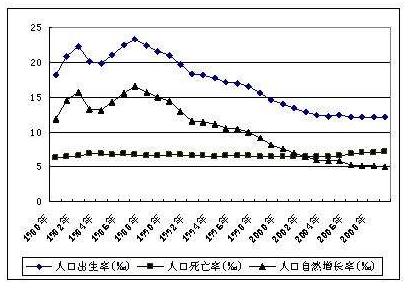
\includegraphics[width=10cm]{Figures/example_fig_1.png}
    \label{fig: fig_1}
    \bicaption{图名}{Figure title}
\end{figure}

描述旋流-静态微泡浮选柱的旋流场结构\footnote{当论文中的字、词或短语等,需要进一步加以说明,而又没有具有的文献来源时,用注释。},分析旋流场特征及其影响;借助流体力学软件对柱体的内部流场进行模拟并分析其流场速度分布规律,研究循环矿浆量及给矿量等因素对流场的影响;\footnote{当论文中的字、词或短语等,需要进一步加以说明,而又没有具有的文献来源时,用注释。}通过对旋流场内的颗粒受力分析,建立基于旋流的颗粒动力学方程;系统揭示旋流分选作用,并进行相关动力学分析…

……

……

……

……

……

……

……

……

……

……

……

……

……
